\PassOptionsToPackage{countmax}{subfloat}
\makeatletter
\def\caption@documentclass{standard}
\makeatother
\documentclass[gmd, manuscript]{copernicus}

\begin{document}
% Generated from schema-v3/v4 machine artifacts; do not edit by hand.
\newcommand{\ValidationTrials}{300}
\newcommand{\ValidationReferenceRepetitions}{200}
\newcommand{\GaussianCrossingMaximum}{0.0\,\%}
\newcommand{\HeavyTailCrossingRate}{0.3\,\%}
\newcommand{\MultimodalCrossingRate}{0.0\,\%}
\newcommand{\BalancedShiftCrossingRate}{99.3\,\%}
\newcommand{\CfiveLikeShiftCrossingRate}{39.7\,\%}
\newcommand{\MinimumShiftCrossingRate}{32.3\,\%}
\newcommand{\IntervalCoverageMinimum}{91.7\,\%}
\newcommand{\IntervalCoverageMaximum}{95.8\,\%}
\newcommand{\IntervalSeedRepetitions}{24}
\newcommand{\IntervalTargetResamples}{5\,000}
\newcommand{\CorrectBlockReferenceWidth}{0.337}
\newcommand{\FrameIIDReferenceWidth}{0.178}
\newcommand{\GeneratedPerClass}{1\,000}
\newcommand{\GeneratedTotal}{6\,000}
\newcommand{\TrainingFrames}{51\,890}
\newcommand{\TrainingStorms}{2\,761}
\newcommand{\ValidationFrames}{7\,191}
\newcommand{\ValidationStorms}{379}
\newcommand{\TestFrames}{7\,011}
\newcommand{\TestStorms}{368}
\newcommand{\MemorizationTrainingFields}{51\,890}
\newcommand{\ControlReferenceFields}{1\,000}
\newcommand{\CfiveFrames}{85}
\newcommand{\CfiveStorms}{22}
\newcommand{\RealTropicalStormShare}{56.2\,\%}
\newcommand{\RealCategoryFiveShare}{1.2\,\%}
\newcommand{\ControlLaneCount}{17}
\newcommand{\MinimumResolvedCopyFraction}{25\,\%}
\newcommand{\WindSlopeComparisons}{42}
\newcommand{\WindRealResolved}{11}
\newcommand{\WindGeneratedResolved}{20}
\newcommand{\WindBothResolved}{8}
\newcommand{\WindBothSameSign}{8}
\newcommand{\WindCfiveRealResolved}{0}
\newcommand{\WindCfiveGeneratedResolved}{5}
\newcommand{\FeatureRepresentationVariants}{12}
\newcommand{\FeatureRobustnessComparisons}{72}
\newcommand{\FeatureMmdWithinCount}{72}
\newcommand{\FeatureDensityAboveCount}{22}
\newcommand{\FeatureCoverageWithinCount}{72}
\newcommand{\FeatureDiversityAboveCount}{64}


\title{GAUGE v0.2.0: empirical reference calibration for evaluating generated climate fields}

\Author[1][guido.ascenso@cmcc.it]{Guido}{Ascenso}
\Author[1,2]{Andrea}{Castelletti}

\affil[1]{CMCC Foundation -- Euro-Mediterranean Center on Climate Change, Milan, Italy}
\affil[2]{Department of Electronics, Information, and Bioengineering, Politecnico di Milano, Milan, Italy}

\runningtitle{GAUGE v0.2.0}
\runningauthor{Ascenso and Castelletti}

\received{}
\pubdiscuss{}
\revised{}
\accepted{}
\published{}

\firstpage{1}
\maketitle

\begin{abstract}
Generative models are increasingly used to synthesise weather and climate fields,
but their evaluation remains fragmented. Generic image-generation scores have little
physical meaning, whereas application-specific histograms and spectra are often
reported without a reference scale for deciding whether an observed discrepancy is
large relative to finite real-data variability. A structured review of 69
climate-generation studies motivates GAUGE, an open empirical reference-calibration
protocol for unpaired populations of two-dimensional gridded fields. For each
registered metric and condition, GAUGE repeatedly compares event-disjoint subsets of
held-out real data using the same sample size and event-weighting rule applied to the
generated bank. It reports the model discrepancy in native units and locates it on a
descriptive gap scale whose zero is the median real--real discrepancy and whose one is
its 95th percentile. Metric-specific degradations of reserved training fields provide
interpretable signposts and test whether each diagnostic responds to relevant
failures. Synthetic experiments characterize finite-archive behaviour, Monte Carlo
stability, block misspecification, and the loss of resolution in thin strata. We
demonstrate the protocol on \GeneratedTotal{} satellite brightness-temperature fields from a
class-conditional tropical-cyclone diffusion model. The example shows why a single
global comparison can be confounded by class composition, why apparently favourable
physical marginals can coexist with discrepancies in spatial and feature-space
structure, and why results supported by only \CfiveStorms{} Category 5 storms require explicit
qualification. GAUGE does not certify equality or collapse heterogeneous evidence
into a model score; it provides a compact, auditable way to distinguish what was
measured, how it compares with the available real archive, whether the metric detects
known failure modes, and where the data leave the comparison unresolved.
\end{abstract}

\introduction

Generative artificial intelligence is rapidly becoming part of weather and climate
science. Generative adversarial networks and diffusion models are now used to
downscale coarse simulations, reconstruct missing observations, emulate expensive
models, and generate stochastic realizations of high-impact events. Recent
applications include precipitation and radar generation
\citep{survey06,survey17,survey25}, Earth-system emulation
\citep{survey09,survey23}, kilometre-scale atmospheric downscaling
\citep{survey42,survey50}, and probabilistic ensembles for high-impact weather
\citep{survey07,survey43}. Unlike a deterministic forecast, these models are expected
to reproduce a distribution of high-dimensional fields. An evaluation must therefore
ask not only whether a typical image looks plausible, but also whether the model
reproduces the correct range of outcomes, spatial organisation, conditional
behaviour, and rare but scientifically important events.

Image-generation research has largely organized this problem around the Fr\'echet
Inception Distance (FID), which has become the dominant automatic metric for comparing
generative models \citep{Heusel2017,Kynkaanniemi2023}. FID first passes real and
generated images through an Inception-v3 classifier trained on ImageNet. It then
approximates each set of resulting feature vectors by a multivariate Gaussian and
computes the squared 2-Wasserstein distance between their means and covariances. The
metric was attractive because it compares generated images directly with real ones,
responded monotonically to several controlled image corruptions in its original
study, and combines aspects of sample quality and distributional coverage in one
number \citep{Heusel2017}.

Those same design choices also limit what FID can establish. Because the Gaussian
approximation retains only the first two moments of the feature distribution,
differences in multimodality, skewness, or tails can be missed. Ordinary finite-sample
FID is biased, and that bias depends on the model being evaluated, so using the same
number of samples does not in itself guarantee a fair ranking
\citep{Chong2020}. The result also depends on the representation: ImageNet class
structure can influence FID strongly enough that matching ImageNet label frequencies
improves the score without improving perceived image quality
\citep{Kynkaanniemi2023}. Furthermore, apparently minor choices such as image resizing,
anti-aliasing, and compression can materially change the result
\citep{Parmar2022}. Recent experiments have also documented poor sample complexity,
departures from the Gaussian assumption, and disagreement with human judgements in
modern image-generation settings \citep{Jayasumana2024}. These findings do not make
FID useless, but they do mean that it is not a distribution-free measure of realism.
For a geophysical field, an ImageNet feature distance has no direct interpretation in
kelvin, millimetres of rainfall, kilometres of spatial scale, or any other physical
quantity, and a favourable value cannot by itself establish realistic extremes,
spatial spectra, or physical admissibility.

Other machine-learning metrics separate some of the properties that FID combines.
Kernel maximum mean discrepancy (MMD) provides a flexible two-sample distance
\citep{Gretton2012}, while precision--recall and density--coverage diagnostics
distinguish fidelity from support and diversity
\citep{Kynkaanniemi2019,Naeem2020}. They are valuable additional tools, but their
meaning still depends on the chosen feature representation. At the opposite extreme,
climate studies often compare physically meaningful histograms, radial profiles,
spectra, or pixel-level errors. These diagnostics can reveal a wrong temperature
distribution or missing spatial scales, yet a visual overlap between two curves has
no stated uncertainty, a marginal histogram can hide class-specific failures, and
none of these checks necessarily reveals mode collapse or the replay of training
examples \citep{Somepalli2023,Carlini2023}. Thus neither a generic computer-vision
score nor a collection of uncalibrated physical plots provides a complete evaluation.

Interpretability is a separate and equally important problem. Two finite samples of
real climate events will never produce exactly the same histogram, spectrum, or metric
value, even when they come from the same population. Their disagreement depends on the
sample size and, crucially, on the number of genuinely independent events. For
example, 1000 satellite images from 20 tropical cyclones do not contain the same
amount of independent information as 1000 images from 1000 different storms. A raw
model--real distance therefore has no obvious scale: the reader cannot tell whether it is negligible or unmistakably large. For example, a 2\,K Wasserstein
distance in minimum cloud-top temperature could be negligible if equally sized real
samples routinely differ by 3\,K, but compelling evidence of model error if they
usually differ by only 0.2\,K. A visual statement that curves ``overlap well'' has the
same weakness in less quantitative form. Computer-vision benchmarks partly solve this interpretation problem through repeated
use. Models evaluated on the same curated datasets, such as ImageNet, inherit a
history of published FID values that provides evolving signposts for competitive
performance. Although the use of AI is evolving rapidly within climate and weather applications  \citep{Ascenso2026}, these fields remain fragmented into different subfields that each use
different observations, variables, regions, resolutions, and bespoke pre-processing
pipelines. A new climate generator can therefore rarely be compared with a long line
of predecessors evaluated on the same analysis-ready dataset. Interpretation must be constructed from the data available within the study itself.

This need for context has a close precedent in hydrological modelling. Rather than
interpreting an efficiency score in isolation, \citet{Seibert2018} compare it with an
upper benchmark obtained from a well-calibrated bucket model and a lower benchmark
obtained from an ensemble of uncalibrated parameterizations. The resulting interval
expresses what could reasonably be achieved and what should be expected at minimum
under the same forcing. The principle is compelling, but it cannot be transferred
literally to general-purpose generative models. There is no climate-wide equivalent of
a bucket model, no canonical ``uninformed'' generator, and no single form of
degeneracy: a model can be too smooth, physically shifted, mode-collapsed, or copied
from its training set. These failures affect different metrics and can be arbitrarily
severe, so they cannot define a universal lower benchmark or support a meaningful
normalisation of every metric between zero and one.

We postulate that these unresolved choices have prevented the emergence of a shared
minimum standard for evaluating generated climate fields. We first examine this claim
through a structured review of a curated corpus of 69 peer-reviewed studies, asking how often
authors document a held-out test set, quantify distributional and conditional
fidelity, report uncertainty, establish a real-vs-real reference, assess diversity and
physical admissibility, validate their metrics, and check for memorization. The review,
presented immediately after this introduction, quantifies which parts of the problem
are already addressed routinely and which remain largely absent.

We then introduce GAUGE (Guidelines for the Assessment and Uniform reporting of
Generative Earth-system models). GAUGE transfers the benchmarking principle of
\citet{Seibert2018}, rather than their literal hydrological bounds. For each chosen
metric, it repeatedly compares two independent, equally sized samples of held-out real
events. These comparisons show how much disagreement is unavoidable when the
evaluation is repeated with the available archive. The resulting empirical reference
depends on the observations, sample size, event structure, conditioning, and metric;
it is not an oracle, noise floor, or population-equality test. The generated sample is then compared
with real data under the same sample size, event weighting, and resampling scheme. A
model discrepancy above the 95th percentile is described as
\texttt{ABOVE\_REFERENCE\_RANGE}; a value below it is
\texttt{WITHIN\_REFERENCE\_RANGE} and does not establish equality or acceptability
(Section~\ref{sec:reference}). For a
compact visual summary, GAUGE
defines one ``reference gap'' as the distance from the median real-vs-real discrepancy
to that 95th percentile. The model and several deliberately degraded real
datasets are plotted in the same gap units. The degraded datasets are not claimed to
be a universal lower bound in the sense of Seibert et al.; they are named signposts showing what physically shifted,
blurred, displaced, phase-randomized, or copied data look like to each metric. Raw
values in physical units, reference quantiles, conditional uncertainty, data support,
and control status remain available alongside the summary.

To demonstrate the framework, we evaluate a class-conditional diffusion model that
generates \(256\times256\) infrared brightness-temperature images of tropical
cyclones. The case is demanding because cloud-top temperature, radial organisation,
and spatial texture all change with storm intensity, while the most consequential
Category 5 storms are represented by only \CfiveStorms{} independent events in the
held-out archive. We compare \GeneratedTotal{} generated fields with storm-disjoint
GridSat-B1 observations linked to one-minute sustained-wind estimates from IBTrACS
\citep{Knapp2010,Knapp2011}. The demonstration therefore tests whether GAUGE can
summarize broad model performance without allowing the abundant weak storms to hide
failures in the tail.

The contributions of this work are threefold. First, the structured review
quantifies the fragmentation of current evaluation practice and identifies the
specific reporting gaps that motivate GAUGE. Second, GAUGE provides an interpretable
framework to benchmark generative AI models for climate science applications that works across heterogeneous
metrics. Third, we provide
an open implementation, broad synthetic validation of the empirical calibration
procedure and metric controls, and
a fully auditable tropical-cyclone case study. Figure~\ref{fig:framework} summarizes
the workflow.

\begin{figure}[t]
\centering
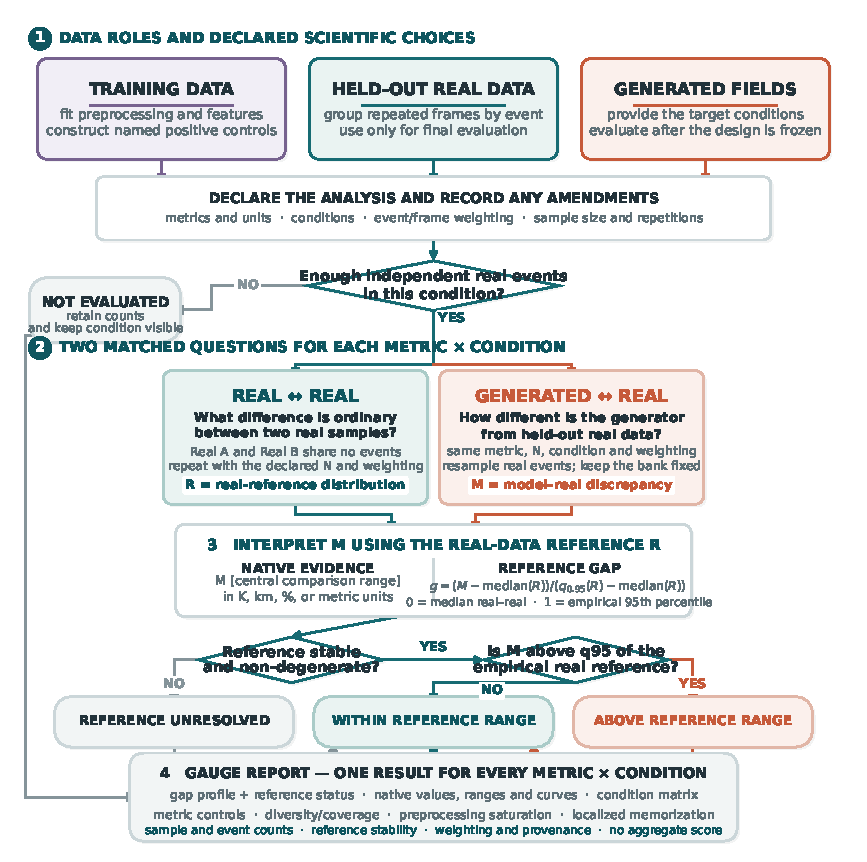
\includegraphics[width=16cm]{fig01.pdf}
\caption{GAUGE workflow. The training data are used only to define preprocessing,
feature representations, and metric-specific controls. Repeated comparisons between
event-disjoint groups of held-out real fields form the empirical real-reference
distribution for each metric, while the generated bank is compared under the same
sample size, condition, and weighting. The report combines a reference-gap profile
with native discrepancies, conditional uncertainty, control responses, independent
event counts, and provenance.}
\label{fig:framework}
\end{figure}

\section{Evidence from a structured literature review}
\label{sec:survey}

\subsection{Corpus and coding}

We conducted a structured review of a curated corpus of 69 peer-reviewed studies
published between 2020 and 2026 whose core focus was developing a generative AI model
for climate, weather, or other geophysical fields. The purpose was to test a specific
hypothesis: that evaluation practices are fragmented and often omit the context
needed to interpret metric values. The corpus was deliberately assembled around that
scope rather than drawn as a probability sample of every climate-generation paper.
Its counts therefore characterize the reviewed evidence base and identify recurring
gaps; they are not presented as prevalence estimates for the entire field.

Each paper was coded against the same questions concerning test-set separation, distributional and
conditional fidelity, extremes, spatial spectra, physical admissibility, diversity,
memorization, metric uncertainty, real-vs-real comparison, and metric validation. For
criteria that admit different levels of evidence, we distinguish an
explicit quantitative assessment from partial evidence, such as a visual comparison
without a reported statistic. Figure~\ref{fig:survey} uses the stricter code: a
practice counts only when it is documented explicitly and, where applicable,
evaluated quantitatively. The complete title and DOI list, criterion definitions,
row-level coding (including partial codes), and candidate log are distributed in the
paper's data archive and repository so that every count can be inspected and
reproduced.
\nocite{survey01,survey02,survey03,survey04,survey05,survey06,survey07,survey08,survey09,survey10,
survey11,survey12,survey13,survey14,survey15,survey16,survey17,survey18,survey19,survey20,
survey21,survey22,survey23,survey24,survey25,survey26,survey27,survey28,survey29,survey30,
survey31,survey32,survey33,survey34,survey35,survey36,survey37,survey38,survey39,survey40,
survey41,survey42,survey43,survey44,survey45,survey46,survey47,survey48,survey49,survey50,
survey51,survey52,survey53,survey54,survey55,survey56,survey57,survey58,survey59,survey60,
survey61,survey62,survey63,survey64,survey65,survey66,survey67,survey68,survey69}

\subsection{What current practice reveals}

Figure~\ref{fig:survey} reveals a marked asymmetry between experimental separation and
metric interpretation. Held-out testing is nearly universal in the reviewed corpus,
and conditional or tail-focused analyses are common. The less common practices form two connected gaps. First, quantitative physical or
distributional diagnostics are seldom accompanied by uncertainty or a real-vs-real
reference. A reported histogram distance may therefore be reproducible yet still
uninterpretable: its sampling variability is unknown, and the reader cannot tell
whether two equally sized real samples would differ by a similar amount. Second,
checks aimed specifically at generative failure modes (e.g.,support loss, excessive
dispersion, physically inadmissible output, insensitive metrics, and training-data
replay) are not routinely combined with physical diagnostics. Consequently, strong
agreement in several marginals can coexist with undetected mode collapse, copying, or
structural failure. 

\begin{figure}[t]
\centering
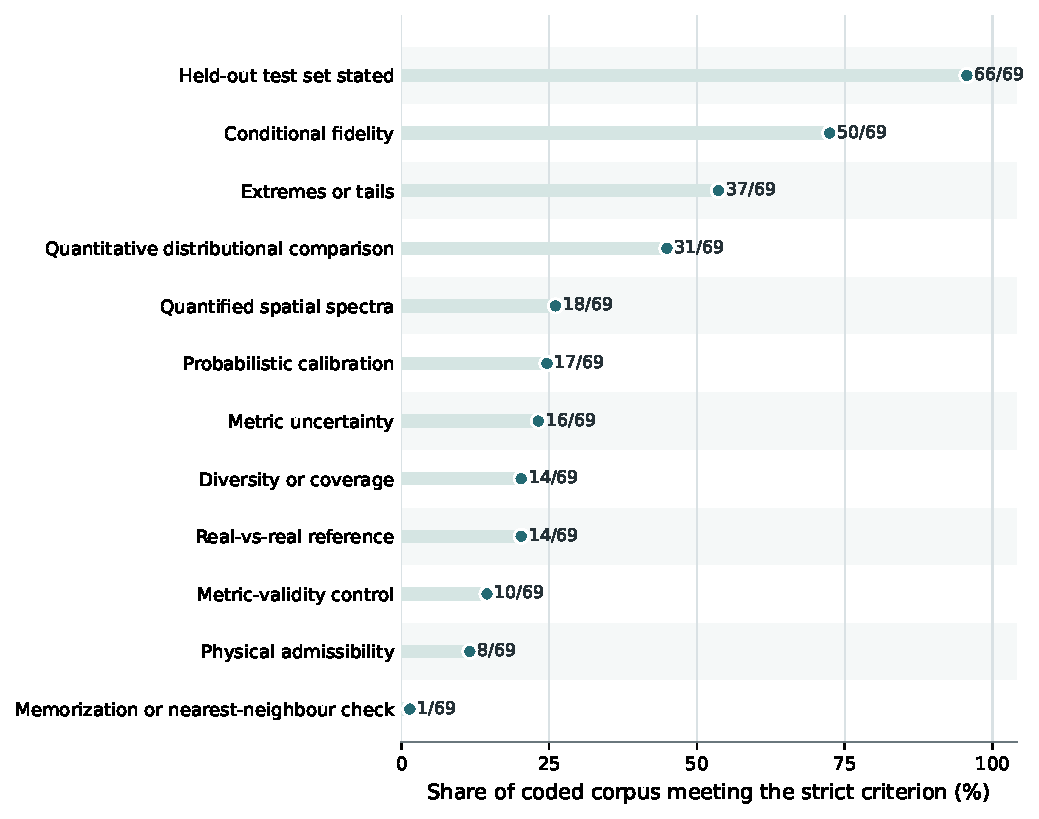
\includegraphics[width=16cm]{fig02.pdf}
\caption{Evaluation practices documented in the structured review
(\(n=69\)). A paper is counted only when the criterion is stated explicitly or
evaluated quantitatively; partial and visual-only evidence is retained in the
archived row-level coding but is not included in the plotted count.}
\label{fig:survey}
\end{figure}

We do not claim to have found that individual studies are uniformly weak, nor that every
criterion is necessary in every application. Rather, each paper tends to assemble a
different subset of otherwise valid diagnostics. This makes results difficult to
compare and leaves no shared evidential standard for deciding whether a reassuring
metric is precise, informative, and sensitive to the failure it is meant to reveal. The central finding is that evaluation metrics are rarely connected by a shared
interpretation.
Physical diagnostics, feature-space distances, conditional checks, uncertainty, and
generative failure tests appear in different combinations, while the reference needed
to interpret the results is absent in most of the corpus. GAUGE
is designed around this specific gap: it preserves application-relevant metrics, adds
a common real-vs-real benchmark to provide interpretability, and makes uncertainty, positive controls, diversity,
admissibility, and memorization explicit rather than leaving them to ad hoc reporting.

\section{GAUGE: philosophy and evaluation protocol}
\label{sec:protocol}

\subsection{What the protocol is intended to add}

GAUGE is an empirical calibration layer around scientifically chosen diagnostics. It
does not replace the quantities that specialists already use, and it does not combine
them into a model score. Instead, it asks four linked questions. Which properties of
the generated fields matter scientifically? How large is each model--real discrepancy
in its natural unit? How does that discrepancy compare with the variation obtained
when the same finite archive is divided into event-disjoint real samples? Finally, does
the metric respond to a known failure of the kind it is intended to reveal?

This follows the benchmark philosophy of \citet{Seibert2018}, but not their literal
upper and lower hydrological bounds. A general generative model has no analogue of a
single well-calibrated bucket model and no unique worst case. A generator can be
shifted, over-smoothed, mode-collapsed, over-dispersed, spatially disorganised, or
partly copied from training data. GAUGE therefore uses two empirical anchors. Repeated
real--real comparisons provide a study-specific reference distribution, and
deliberately altered real fields show how named failures affect each metric. Neither
anchor defines scientific acceptability, and the evidence remains disaggregated by
metric and condition.

Version 0.2 addresses unpaired sample-to-population fidelity for independent
single-channel or multichannel two-dimensional gridded fields. It is not a forecast
verification framework. Proper scores such as CRPS, reliability diagrams, rank
histograms, scale-aware scores such as FSS, object-based scores such as SAL, and
benchmark suites such as WeatherBench address paired forecasts, ensemble calibration,
location error, or common predictive tasks \citep{GneitingRaftery2007,Hamill2001,
RobertsLean2008,Wernli2008,Rasp2020}. Those methods remain necessary when such
questions are present. Trajectories, downscaling pairs, irregular observations, and
coupled systems similarly need complementary verification or future adapters.

\subsection{Data roles, independent events, and weighting}

The protocol distinguishes three data sources. \(X_{\mathrm{train}}\) contains the
real fields that were available while the generator and any data-derived evaluation
components were fitted. \(X_{\mathrm{real}}\) is the held-out archive used for the
final comparison. \(X_{\mathrm{gen}}\) is the fixed generated bank being evaluated.
Real and generated fields must represent the same variables, units, grid, processing,
and conditioning labels.

Several fields may describe the same physical event and are then not independent.
The software calls the event label a \emph{block identifier}. A block is simply the
unit that must remain intact during resampling: a tropical cyclone in this study, but
potentially a weather system, simulation member, station, or year in another
application. At each repetition, complete blocks are divided into two non-overlapping
groups. No storm can therefore contribute images to both real samples. Choosing the
scientifically correct block is the user's responsibility; treating correlated frames
as independent makes the reference artificially narrow.

The weighting rule defines which real-field population is being summarized. The
default gives every block the same total weight. If block \(b\) contains \(n_b\)
eligible frames \(x_{bi}\), its empirical distribution is

\begin{equation}
\widehat{P}_{\mathrm{block}} =
\frac{1}{B}\sum_{b=1}^{B}\frac{1}{n_b}\sum_{i=1}^{n_b}\delta_{x_{bi}} .
\label{eq:blockbalanced}
\end{equation}

Thus a storm is selected uniformly and a frame is then selected within that storm.
A frequently observed storm cannot dominate only because it contributes more
images. A frame-weighted alternative is available when the distribution of recorded
frames is the intended target. The selected rule, condition, and sample size are
identical for the two real samples and the model--real comparison. Conditional
generators should normally be evaluated within each native condition. A pooled result
is a fidelity comparison only when the real and generated condition mixtures match;
otherwise it is a dataset-composition audit.

\subsection{Physical quantities and complementary diagnostics}

The scientific core is a short, documented set of scalar quantities. For the TC
application these include cloud-top temperatures, cold-cloud area, radial scale, and
storm organisation. For scalar quantity \(f_j(X)\), GAUGE uses the one-dimensional
Wasserstein-1 distance

\begin{equation}
W_1(P_j,Q_j) =
\int_0^1\left|F_j^{-1}(u)-G_j^{-1}(u)\right|\,\mathrm{d}u ,
\label{eq:w1}
\end{equation}

where \(F_j^{-1}\) and \(G_j^{-1}\) are empirical quantile functions
\citep{Villani2009}. The result has the same unit as \(f_j\) and can be read as the
average displacement required to align the two scalar distributions. This common
estimator does not make a kelvin commensurate with a kilometre; scientific magnitude
is still read from the native value.

Scalar marginals cannot reveal every generative failure. The registry can therefore
also contain curve discrepancies, spatial spectra, MMD, density, coverage, diversity,
preprocessing audits, and training-sample similarity
\citep{Gretton2012,Naeem2020}. In v0.2 the Gaussian-kernel MMD uses the non-negative
biased V-statistic. The radial-spectrum discrepancy is the mean squared difference
between log-base-10 power curves and has units of dex\({}^2\). Every metric records
its preprocessing, orientation, units, and data provenance.

Some supporting metrics operate on a lower-dimensional representation of the fields.
In this study, physical quantities are standardized and concatenated with empirical
orthogonal function (EOF) coefficients. The standardization, EOF patterns, component
scales, kernel bandwidth, and neighbourhood definitions are all fitted using training
data. This prevents the held-out archive from being used to construct a favourable
representation. Users may instead supply an independently trained representation,
but must record the data and procedure used to obtain it.

\subsection{The empirical real-reference distribution}
\label{sec:reference}

For metric \(d\), condition \(c\), and declared evaluation size \(N\), repetition
\(k\) divides eligible held-out blocks into disjoint groups \(A_k\) and \(B_k\).
GAUGE samples \(N\) fields from each group using the declared weighting rule and
computes

\begin{align}
R_k &= d(X^{(k)}_{\mathrm{real},A},X^{(k)}_{\mathrm{real},B}),\\
M_k &= d(X^{(k)}_{\mathrm{gen}},X^{(k)}_{\mathrm{real},B}).
\label{eq:reference}
\end{align}

The paired sequences \(\{R_k,M_k\}\) are stored. The first is the
\emph{real-reference distribution}: the discrepancies obtained between event-disjoint
real subsets under this particular archive, sample size, weighting, and condition.
The second records how the fixed generated bank compares with the admissible real
subsets. The reported model discrepancy is the median of \(M_k\), accompanied by a
central comparison range across those subsets.

The real-reference median \(q_{0.50}^{RR}\) represents typical disagreement between
the matched real samples, and \(q_{0.95}^{RR}\) marks the upper 5\,\% of that empirical
distribution. GAUGE labels a result \texttt{WITHIN\_REFERENCE\_RANGE} when the median
model discrepancy is no larger than \(q_{0.95}^{RR}\), and
\texttt{ABOVE\_REFERENCE\_RANGE} when it is larger. These labels are descriptive.
The reference is not a noise floor or an oracle. It is not a population-equality
distribution or an exact level-\(\alpha\) procedure. In particular,
\texttt{WITHIN\_REFERENCE\_RANGE} does not establish equality, equivalence, or
scientific adequacy. It says only where this result lies relative to the empirical
variation created by the declared evaluation design.

Metrics with different units cannot share a native axis. GAUGE therefore uses the
reference gap

\begin{equation}
g =
\frac{\widetilde{M}-q_{0.50}^{RR}}
{q_{0.95}^{RR}-q_{0.50}^{RR}},
\label{eq:gap}
\end{equation}

where \(\widetilde{M}=\operatorname{median}_k M_k\). On this presentation scale,
\(g=0\) is the median real-reference discrepancy and \(g=1\) is its 95th percentile.
A negative value means that the model comparison is smaller than the median
real--real comparison; it does not mean ``better than real'' and may also arise from
an under-dispersed generator. The gap depends on the archive, sample size, condition,
weighting, and metric. It is neither physical severity nor an aggregate model score.
GAUGE therefore always presents it beside the native discrepancy and the reference
quantiles. Degraded-data controls appear on the same axis only as labelled signposts
of concrete failure mechanisms.

\subsection{Uncertainty and limited reference resolution}

Three uncertainties must not be conflated. First, the central comparison range of
\(M_k\) describes variation over admissible held-out real subsets while the generated
bank remains fixed. It does not include a new generator fit, another model checkpoint,
or another observational archive. Second, GAUGE uses a paired bootstrap of the stored
\((R_k,M_k)\) repetitions to summarize Monte Carlo uncertainty in
\(q_{0.50}^{RR}\), \(q_{0.95}^{RR}\), and \(g\). These conditional intervals describe
the numerical precision of the empirical summaries, not physical tolerance. Third,
archive uncertainty is assessed separately by deleting groups of complete real
blocks; it cannot be created by drawing more frames from the same events.

The reference can be too weak to interpret. GAUGE returns
\texttt{REFERENCE\_UNRESOLVED} when the denominator in Eq.~(\ref{eq:gap}) is
degenerate or when the estimated reference quantile is unstable across the
resampling sequence. \texttt{NOT\_EVALUATED} is reserved for invalid data or an
unsupported metric. These fail-closed states are especially important for conditions
with few independent events. Version 0.2 makes no familywise, multiplicity-adjusted,
or aggregate pass/fail statement: every metric--condition result describes a
different scientific property and is interpreted on its own.

\subsection{Metric-specific controls and training-data copying}

A small gap is reassuring only if the metric can respond to the failure it is meant
to diagnose. Controls are therefore registered by metric and constructed from
reserved training events. Their full severity curves are reported. Examples include
adding 0.5, 1, 2, and 4\,K to reserved fields for lower-tail temperature metrics,
warming and cooling pixels around a registered threshold, progressive blur for
spatial power, removal of feature-space modes for coverage,
contraction or expansion for diversity, and artificial boundary spikes for the
preprocessing saturation audit. A Fourier-phase control deliberately disrupts storm
organisation while preserving each field's unwindowed discrete Fourier magnitudes;
organisation metrics should therefore respond without attributing that response to a
change in the unwindowed spectrum. Because the registered spectrum is computed after
Hann windowing, its separate invariance control is a 90\(^\circ\) field rotation.

The control registry distinguishes four outcomes. \texttt{CONTROL\_VALIDATED} means
that the expected severity response and any declared invariance check were observed.
\texttt{RESPONSIVE\_BELOW\_REFERENCE\_RANGE} means that the metric moved as expected
but the tested severities remained inside the empirical reference range.
\texttt{CONTROL\_FAILED} withholds an affirmative interpretation while leaving the
raw model result visible. \texttt{CONTROL\_NOT\_REGISTERED} makes the absence of a
control explicit. A single overall ``passed'' label is not produced.

Training replay is checked separately because a small copied fraction can disappear
inside a dataset-wide average \citep{Somepalli2023,Carlini2023}. GAUGE maps training,
held-out, and generated fields into the training-fitted feature representation and
partitions that space into fixed neighbourhoods. Within every sufficiently populated
class--neighbourhood combination it compares generated-to-training nearest-neighbour
distances with held-out-real-to-training distances. Generated samples that are
systematically closer are flagged descriptively as
\texttt{CLOSER\_TO\_TRAINING}; storm bootstrap resampling supplies the held-out
comparison range. Exact training replay and mixtures containing 1, 5, 10, 25, 50,
and 100\,\% copied fields establish the resolution of this audit. The result applies
only to the registered representation and supported neighbourhoods; it cannot rule
out every possible form of memorization.

\section{Software implementation}
\label{sec:software}

GAUGE is implemented as the BSD-3-Clause Python distribution
\texttt{gauge-climate}, with import namespace
\texttt{gauge\_\allowbreak climate}. Stable public
objects describe the three datasets, physical quantities, supporting metrics,
evaluation settings, and final report. NumPy arrays and memory-mapped arrays are core
inputs, while an optional xarray adapter accepts labelled scientific arrays and records
when lazy data are loaded into memory. The implementation uses NumPy, SciPy, and
Matplotlib \citep{Harris2020NumPy,Virtanen2020SciPy,Hunter2007}.

The software checks the scientific assumptions before running an evaluation and
rejects samples that appear in both training and test data, missing event identifiers,
label arrays that do not contain exactly one correctly ordered label per field,
unsupported missing values, incompatible
shapes or units, conditions with fewer than twice the configured events-per-half
minimum,
and feature representations whose parameters were estimated from the test set. For every
metric--condition comparison, the report records the native discrepancy and central
comparison range, units, real-reference median and 95th percentile with conditional
Monte Carlo intervals, reference percentile and gap with its interval, sample and
event counts, weighting rule, reference and control status, warnings, random seeds,
software versions, and preprocessing history. A schema-v3 JSON file is the
authoritative record; figures, HTML, and tables are generated from that object.
Version 0.2.0 reads older reports through a one-way migration while writing only
\texttt{gauge\_climate.evaluation.v3}.

\section{Validation of empirical reference calibration}
\label{sec:validation}

Because the reference gap is a new descriptive scale, we examined its behaviour
before using it in the TC demonstration. The purpose was not to prove a universal
error rate. Instead, the experiments ask whether same-population generators usually
remain within the empirical reference range, whether progressively stronger known
changes cross it more often, and when the reference becomes numerically or
scientifically uninformative.

Scalar experiments cover Gaussian, heavy-tailed, and multimodal populations; location
and variance changes; narrowed and widened distributions; tail contamination; and a
training-to-test distribution shift. Six event designs use 80 equally sized blocks at
\(N=80\), 240, and 1000; 80 severely unequal blocks at \(N=240\); 22 blocks at
\(N=1000\); and the operational minimum of 20 blocks at \(N=1000\). We generated
\ValidationTrials{} independent archives per setting and used
\ValidationReferenceRepetitions{} reference repetitions per archive. The reported
\emph{same-population boundary-crossing rate} is the proportion for which a
same-population generator lies above \(q_{0.95}^{RR}\). The
\emph{perturbation crossing probability} is the corresponding proportion after a
known change. Wilson intervals describe Monte Carlo precision of these rates
\citep{Wilson1927}.

Separate spatial and feature-space experiments cover curve MAE and log-power
discrepancy under known spatial-scale changes, and MMD\({}^2\), density, coverage, and
diversity under mode removal, duplication, contraction, expansion, and off-manifold
contamination. We also repeat the reference construction with intentionally
incorrect frame-level identifiers. This does not offer frame-IID resampling as an
alternative; it demonstrates the consequence of ignoring event dependence.

Across the Gaussian settings, the largest same-population crossing rate was
\GaussianCrossingMaximum{}; the corresponding rates were
\HeavyTailCrossingRate{} for the heavy-tailed population and
\MultimodalCrossingRate{} for the multimodal population. Stronger perturbations
crossed more frequently than weaker ones (Fig.~\ref{fig:validation}). For example,
a location shift of 0.55 marginal standard deviations crossed in
\BalancedShiftCrossingRate{} of the 80-block trials, compared with
\CfiveLikeShiftCrossingRate{} in the 22-block design and
\MinimumShiftCrossingRate{} at the 20-block minimum. Drawing 1000 frames therefore
did not compensate for the loss of independent events.

The curve and feature metrics changed monotonically under their registered synthetic
controls, and biased MMD\({}^2\) remained non-negative to numerical precision.
Across \IntervalSeedRepetitions{} independent resampling seeds, the paired-bootstrap
intervals covered their \IntervalTargetResamples-repetition conditional targets in
\IntervalCoverageMinimum{} to
\IntervalCoverageMaximum{} of runs, depending on the summary. Grouped
delete-block calculations remained finite but showed the distinct sensitivity to
archive composition. Degenerate widths, unstable quantiles, and fewer than 20
eligible blocks failed closed. The deliberately incorrect frame-IID analysis
contracted the reference width from \CorrectBlockReferenceWidth{} to
\FrameIIDReferenceWidth{} in the synthetic example,
confirming that additional frames cannot substitute for correctly identified
independent events.

\begin{figure}[t]
\centering
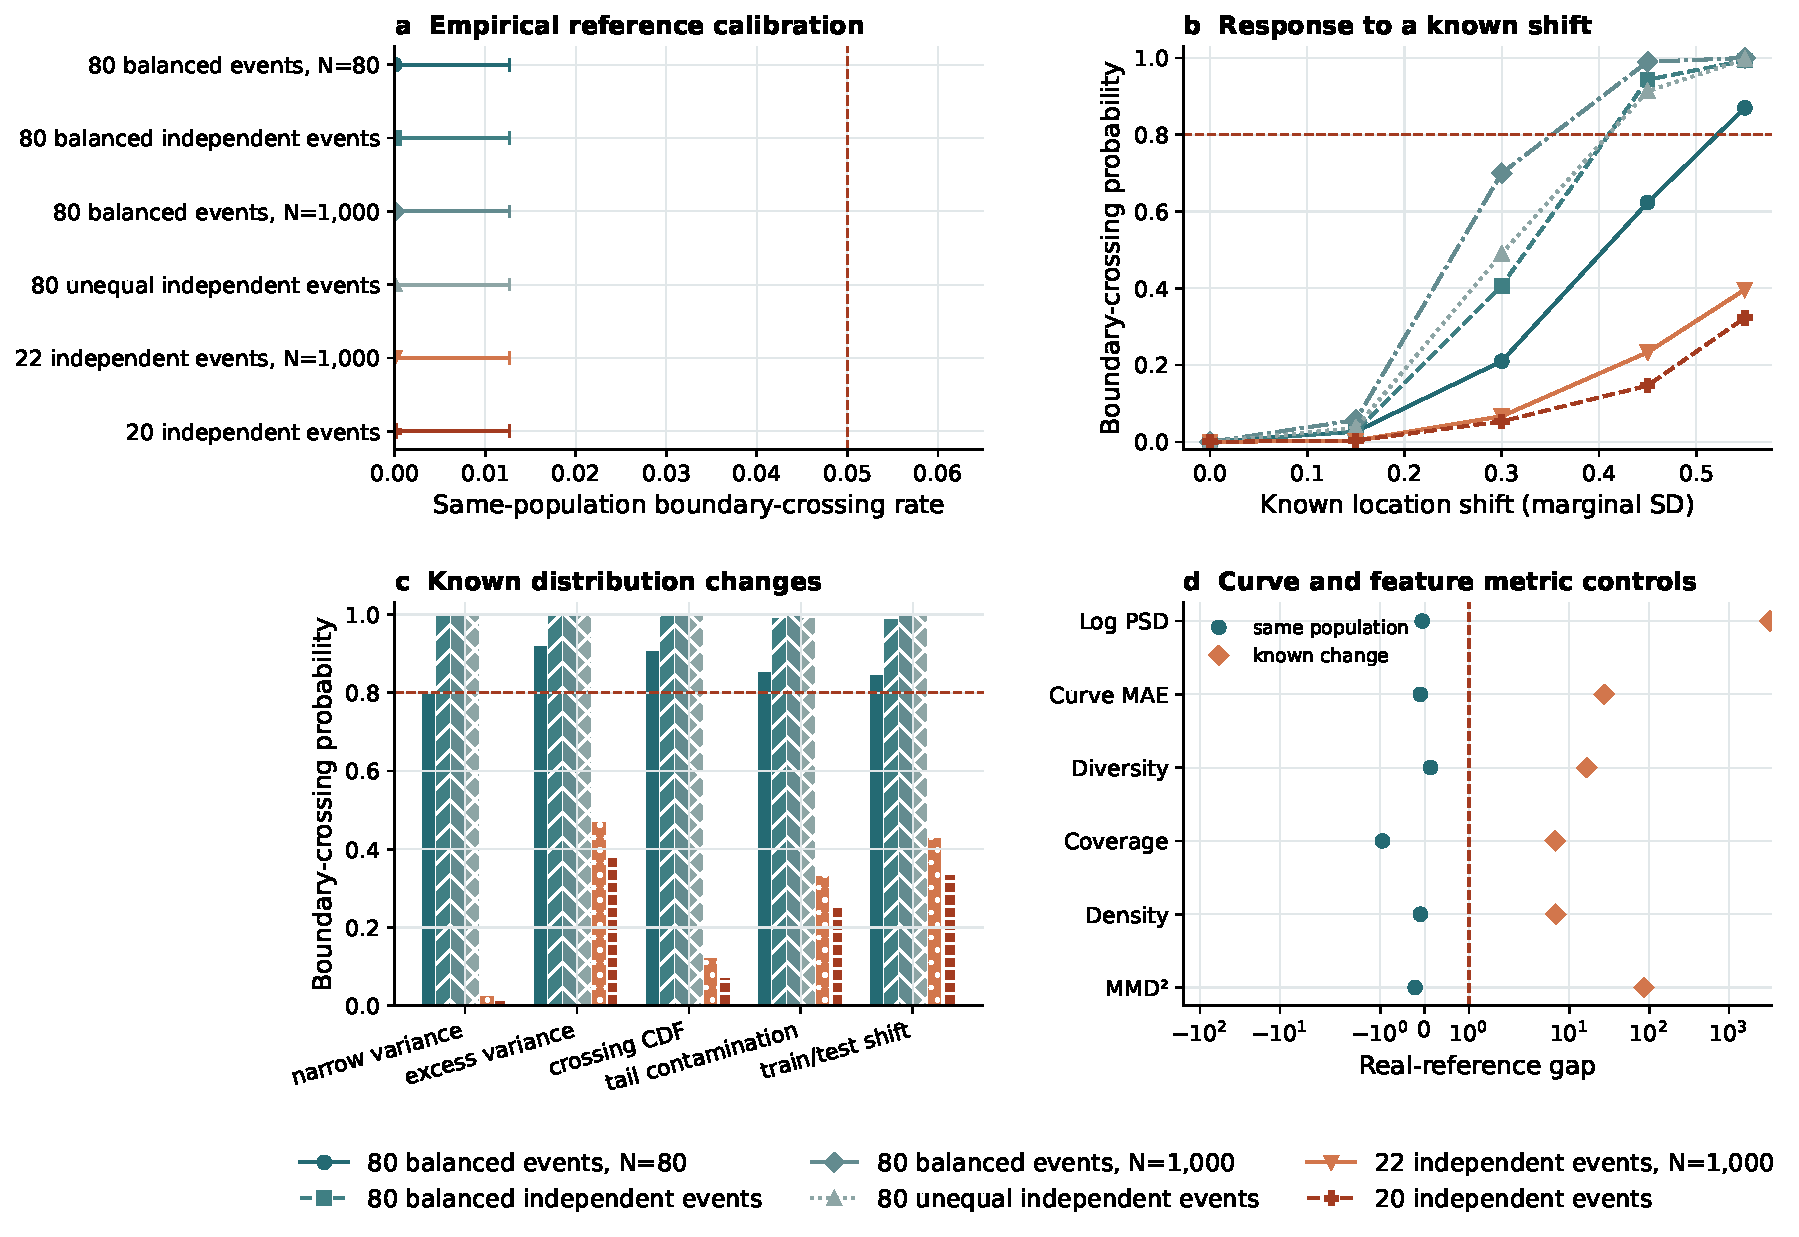
\includegraphics[width=16cm]{fig03.pdf}
\caption{Synthetic validation of the empirical reference calibration. The panels
show same-population boundary-crossing rates, response to increasing perturbations,
the effect of unequal and sparse event support, and reference sensitivity to correct
versus intentionally frame-IID grouping. Bars are 95\,\% Wilson intervals over
\ValidationTrials{}
independent archives where applicable. These experiments characterize the chosen
design; they do not turn the empirical reference into an exact level-\(\alpha\)
procedure.}
\label{fig:validation}
\end{figure}

\section{Tropical-cyclone case study}
\label{sec:tc}

We demonstrate GAUGE by using it to evaluate a conditional diffusion model trained to
generate two-dimensional infrared brightness-temperature fields of tropical cyclones
at specified wind intensities. This application provides a demanding stress-test for GAUGE, because it combines several problems that commonly complicate climate-model evaluation. Specifically, consecutive images from the same storm are not independent, intensity classes are highly imbalanced, and the scientifically important Category 5 tail contains very few storms. Moreover, images that are perceptually realistic (as measurable with traditional metrics from the computer vision literature) may still reproduce the wrong temperature distribution, spatial organisation, variability, or intensity dependence, or may simply copy training examples. The case study therefore exercises GAUGE's main capabilities simultaneously: accounting for event dependence, separating overall from condition-specific performance, evaluating both physical and statistical properties, checking for memorisation, and establishing through metric-specific controls how the selected diagnostics respond to known failures.


The demonstration is not intended to establish a
universal set of TC metrics. Instead, it shows how application-specific physics,
spatial structure, data imbalance, diversity, and memorization can be combined and
interpreted within the same reference framework.

\subsection{Data and partitions}

The data with which we train our generator are global, storm-centred infrared brightness-temperature fields from
GridSat-B1 \citep{Knapp2011} from 1980 to 2025, paired with intensity metadata from IBTrACS
\citep{Knapp2010}. Fields are \(256\times256\) pixels at 8\,km spatial resolution, corresponding to a storm-centred domain approximately 2048 km across. The domain therefore captures the cyclone-scale cloud shield even for the largest storms, as  well as the surrounding environment. All intensity
labels and continuous maximum-wind conditions use one-minute sustained wind, and exclude storms that only ever reached tropical depressions status in their lifetime.

Storm-disjoint train, validation, and test partitions contain
\TrainingFrames{}, \ValidationFrames{}, and \TestFrames{} frames from
\TrainingStorms{}, \ValidationStorms{}, and \TestStorms{} storms, respectively
(Table~\ref{tab:partitions}).
The rarity of the most intense storms creates a particularly difficult challenge for
evaluating the generative model: the Category 5 test data contain \CfiveFrames{}
images from only \CfiveStorms{} storms.

\begin{table*}[t]
\caption{Storm-disjoint TC partitions by intensity class. Storm counts are the number
of storms contributing at least one frame to the class and therefore do not sum to
the split total, as one storm can cross several classes.}
\label{tab:partitions}
\centering
\begin{tabular}{lrrrrrr}
\tophline
& \multicolumn{2}{c}{Train} & \multicolumn{2}{c}{Validation} &
\multicolumn{2}{c}{Test}\\
\cline{2-7}
Class & Frames & Storms & Frames & Storms & Frames & Storms\\
\middlehline
TS & 28\,347 & 2\,747 & 3\,943 & 377 & 3\,942 & 368\\
C1 & 10\,576 & 1\,586 & 1\,498 & 223 & 1\,318 & 211\\
C2 & 5\,265 & 1\,061 & 661 & 150 & 700 & 149\\
C3 & 3\,547 & 800 & 489 & 114 & 505 & 106\\
C4 & 3\,508 & 561 & 509 & 79 & 461 & 76\\
C5 & 647 & 159 & 91 & 23 & 85 & 22\\
\bottomhline
\end{tabular}

\end{table*}

\subsection{Generator and generated bank}

We refer to the evaluated generator as the TC brightness-temperature diffusion model.
It is a conditional
denoising diffusion model \citep{Ho2020,Karras2022} whose U-Net has base width 32, six
resolution levels, three residual blocks per level, and attention at 16- and 32-pixel
resolutions. Training used at most 100 epochs of 2000 steps, a cosine 1000-step
diffusion schedule \citep{Nichol2021}, zero-terminal signal-to-noise rescaling with
\(v\)-prediction \citep{Lin2024}, minimum-SNR weighting with \(\gamma=2.5\)
\citep{Hang2023}, dynamic thresholding \citep{Saharia2022}, and exponential
moving-average weights. The model is conditioned on both intensity class and
continuous USA\_WIND. Its checkpoint was selected using validation loss, without
examining the final GAUGE comparisons.

The sample bank was generated once before the final evaluation and contains
\GeneratedPerClass{} fields per class, for \GeneratedTotal{} fields in total.
Samples were produced from the selected moving-average checkpoint using DPM-Solver++
2M \citep{Lu2023}, 250 trailing timesteps, and guidance scale = 1. Within each
class, continuous wind conditions were sampled to match the corrected held-out
distribution. The generated bank covers 6--12 distinct wind values per class, and the
total-variation distance between generated and real wind distributions ranges from
0.012 to 0.055 (Table~\ref{tab:vmax}). Figure~\ref{fig:examples} uses a deterministic
selection rule so that the displayed fields are representative examples rather than
hand-picked successes.

\begin{figure}[t]
\centering
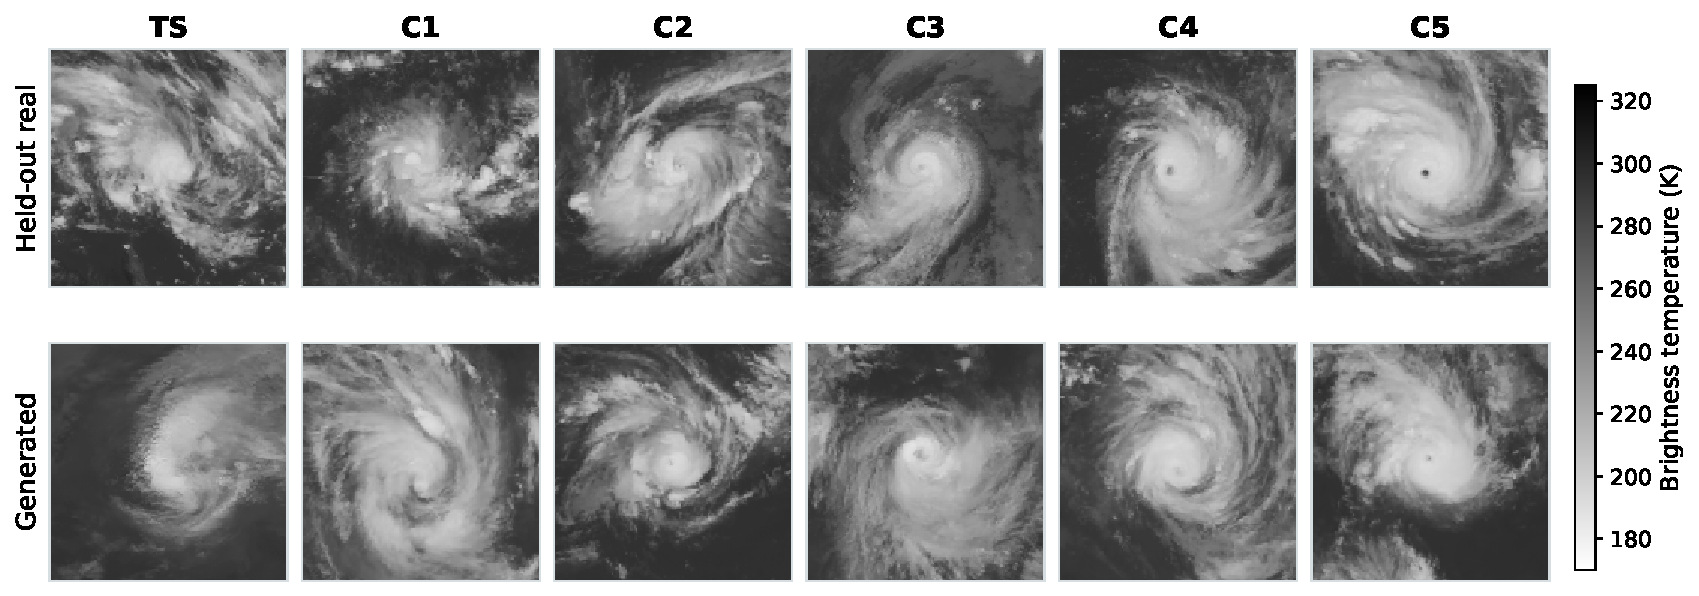
\includegraphics[width=16cm]{fig04.pdf}
\caption{Deterministically selected typical held-out real (top) and generated (bottom)
brightness-temperature fields for TS and Categories 1--5. The selection rule minimizes
distance to the class median across the seven physical quantities used in the
evaluation; it was not based on visual preference.}
\label{fig:examples}
\end{figure}

\begin{table*}[t]
\caption{Continuous wind support in the generated bank and held-out real data. TV is
the total-variation distance between the discrete within-class wind
distributions.}
\label{tab:vmax}
\centering
\begin{tabular}{lrrrrrc}
\tophline
Class & Generated values & Real values & Generated median (kt) & Real median (kt) & TV & Generated support within real\\
\middlehline
TS & 12 & 13 & 45 & 45 & 0.031 & yes\\
C1 & 7 & 7 & 70 & 70 & 0.012 & yes\\
C2 & 6 & 6 & 90 & 90 & 0.020 & yes\\
C3 & 6 & 6 & 105 & 105 & 0.015 & yes\\
C4 & 8 & 8 & 120 & 120 & 0.031 & yes\\
C5 & 9 & 9 & 140 & 140 & 0.055 & yes\\
\bottomhline
\end{tabular}

\end{table*}

\subsection{Case-specific evaluation choices}

The method and this case study were developed iteratively. We therefore provide a
versioned analysis protocol and amendment log rather than describing the exercise as
an untouched confirmatory evaluation. The v0.2 definitions below were fixed before a
complete clean rerun, but the test archive had already informed earlier versions of
GAUGE. This distinction is part of the provenance record.

The seven physical quantities are minimum core brightness temperature within 100\,km, cold-cloud area below
220\,K within 300\,km, radius of the largest azimuthal-mean temperature gradient,
root-mean-square azimuthal departure within 300\,km, deviation-angle variance within
300\,km, eye-to-eyewall temperature contrast, and the first percentile of each field's
brightness temperature (see the Supplement for complete definitions).
Deviation-angle variance follows established uses of infrared
gradient organisation in TC analysis \citep{Pineros2008,Ritchie2012}. These choices
provide diagnostics for the present demonstration; they are not proposed as a
universal TC metric suite.

We complemented the physical distributions with a 32-bin radial
brightness-temperature profile and a 24-shell radial power spectrum, together with
MMD\(^2\), density, coverage, and relative diversity in a 20-component EOF feature
representation. The spectral calculation removes each field's mean, applies a
separable Hann window with energy normalisation, and bins power by physical
wavenumber; its discrepancy is the mean squared difference in log-base-10 power and
is reported in dex\({}^2\). The Gaussian-kernel MMD\({}^2\) uses the non-negative
biased V-statistic. We also examine nearest-neighbour evidence of training-data copying,
relationships among the physical quantities, and saturation at the preprocessing
limits of 170 and 325\,K. These are the fixed bounds used by the generator's
preprocessing pipeline, not physical admissibility limits. The EOF representation was
estimated from 512 training fields, and
feature-set metrics used 256 matched samples in each reference repetition.

Each storm receives equal total weight in the primary analysis, so a storm with many
satellite frames cannot dominate one with few. All six intensity classes are evaluated
separately. No C4+ or other tail aggregate is included: Category 5 remains a native
condition with its limited \CfiveStorms-storm support visible.

The seven physical distributions are evaluated using 2000 real-vs-real repetitions, while curve and feature metrics use 1000 repetitions---except feature coverage, which uses
2000. These budgets were selected during method development to stabilize empirical
reference quantiles; the feature metrics are substantially more expensive per
repetition. The generated bank contains
equal numbers from all six classes, whereas \RealTropicalStormShare{} of the real test
fields are tropical storms and only \RealCategoryFiveShare{} are Category 5. A pooled
comparison would therefore
combine model quality with this large difference in class composition. We base the
fidelity conclusions on the six native within-class comparisons and retain the
unmatched pooled result only as a dataset-composition audit.

Metric-specific controls use reserved training storms. They include additive
temperature shifts, threshold-localized warming and cooling, eye and eyewall
perturbations, displacement, blur, radial
deformation, phase randomisation and a rotational invariance check, mode removal,
feature contraction and expansion, off-manifold artifacts, preprocessing-boundary
spikes, and copied-training fractions from 1 to 100\,\%. For every control we report
the complete severity curve, monotonicity, first boundary-crossing severity, and any
declared invariance property.

Two post-hoc audits examine conclusions that are not captured by the six discrete
classes. First, within each class we estimate the slope of each physical quantity
against the continuous wind condition. Real slopes use inverse storm-frequency
weights and storm bootstrap intervals; generated slopes use equal sample weights and
sample bootstrap intervals. The audit is descriptive and has no equivalence label.
Second, we repeat the feature metrics across EOF fit sizes 256, 512, and 1024; ranks
10, 20, and 40; and low-pass representations at specified physical scales. These
analyses test whether a feature-space pattern persists, weakens, or reverses when a
reasonable representation choice changes.

\section{Case-study results}
\label{sec:results}

\subsection{Class-conditional fidelity profile}

Figure~\ref{fig:profile} is the compact, paper-facing summary of the TC evaluation.
Each row is one registered property, and the six filled symbols retain TS and
Categories 1--5 separately. The point is the median model--real discrepancy expressed
on the reference-gap scale; its horizontal segment is the central range obtained as
the fixed generated bank is compared with admissible held-out-real subsets. It is not
a generator-retraining confidence interval. The shaded region from \(g=0\) to \(g=1\)
spans the real-reference median to its 95th percentile. Values beyond \(g=1\) are
labelled \texttt{ABOVE\_REFERENCE\_RANGE}; values inside are labelled
\texttt{WITHIN\_REFERENCE\_RANGE}. Neither label is a significance test or a verdict
on the model as a whole. Open, shape-coded symbols provide selected degraded-real
signposts; the complete severity curves are reported in the Supplement.

\begin{figure}[t]
\centering
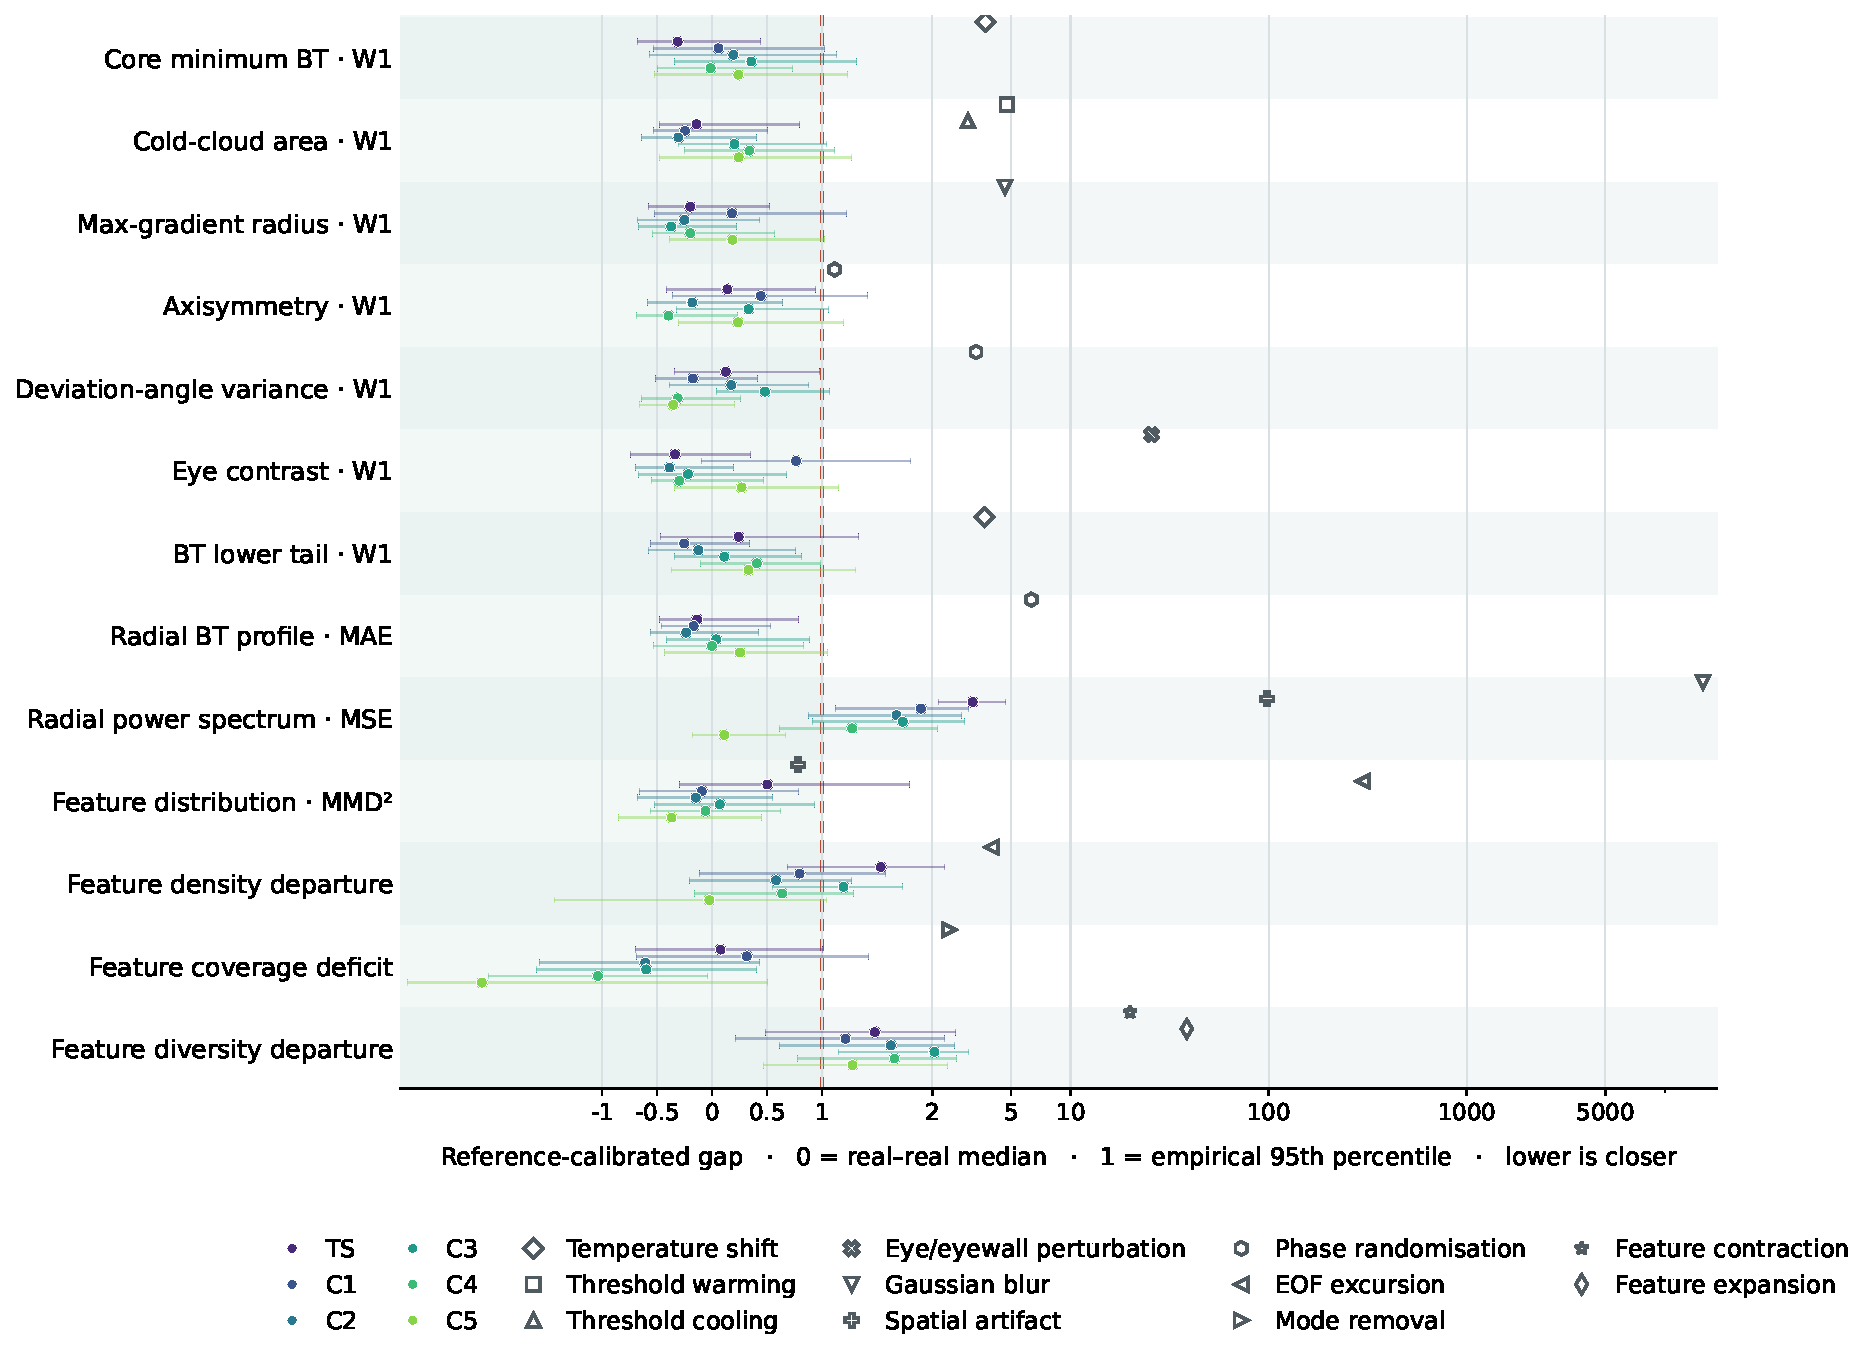
\includegraphics[width=17cm]{fig05.pdf}
\caption{Reference-gap profile for the six native intensity classes and 13 metrics.
Filled, class-specific symbols show model results; horizontal segments show the
central comparison range across admissible held-out-real subsets while the generated
bank remains fixed. The shaded region runs from the real-reference median
(\(g=0\)) to its 95th percentile (\(g=1\)). Distinct open symbols are degraded-real
signposts constructed from reserved training storms. The nonlinear axis preserves
negative gaps and large control responses. The gap is a descriptive coordinate
conditional on this archive and design, not physical severity or a model score.}
\label{fig:profile}
\end{figure}

The selected physical marginals form a coherent favourable pattern: the distributions
of core minimum temperature, cold-cloud area, maximum-gradient radius, axisymmetry,
deviation-angle variance, eye contrast, and lower-tail temperature remain within
their respective reference ranges in every native class. Mean radial profiles show
the same class-wide pattern. These results state that the observed discrepancies are
not unusually large relative to the matched finite-archive real comparisons; they do
not show equality or define a physically acceptable error.

The spatial and feature diagnostics qualify that result. Radial log-power is above
the reference range from TS through Category 4, revealing a scale-dependent
structural difference that is not visible in the seven scalar marginals or the mean
radial profile. Feature MMD\({}^2\) and coverage remain within range across the native
classes. Feature density is above range for TS and Category 3, while the diversity
departure is above range throughout the intensity ladder; its signed companion
identifies larger, rather than collapsed, mean pairwise feature distances. The
generator therefore matches the selected physical distributions more closely than it
matches spatial texture and feature-space dispersion. Native discrepancies,
reference summaries, Monte Carlo intervals, statuses, and warnings are tabulated in
the Supplement.

The pooled comparison provides a separate demonstration of why conditioning matters.
The generated bank assigns one sixth of its samples to every class, whereas tropical
storms make up \RealTropicalStormShare{} of the real test images and Category 5 storms
only \RealCategoryFiveShare{}.
When all classes are combined, every selected physical marginal lies above its
real-reference range. This result reflects the intentionally balanced
generated mixture versus the naturally imbalanced observed mixture, not a failure to
generate the physical distribution within a given class. The within-class results are
therefore the basis for the fidelity interpretation; the pooled row is retained only
as a dataset-composition audit.

\subsection{What can be said about Category 5}

The tail deserves a separate reading because it is scientifically consequential and
has the weakest observational support. Category 5 contributes only \CfiveFrames{}
held-out frames from \CfiveStorms{} storms. Figure~\ref{fig:c5dist} therefore shows
the complete event-balanced distributions rather than hiding the condition in a
pooled C4+ statistic. The seven physical discrepancies remain within their empirical
reference ranges, but their broad central comparison ranges show that materially
different subsets of the small real archive can yield different model--real
distances. The native-unit values and conditional Monte Carlo intervals are provided
in the Supplement so that the compact gaps are not read without their scale.

\begin{figure}[t]
\centering
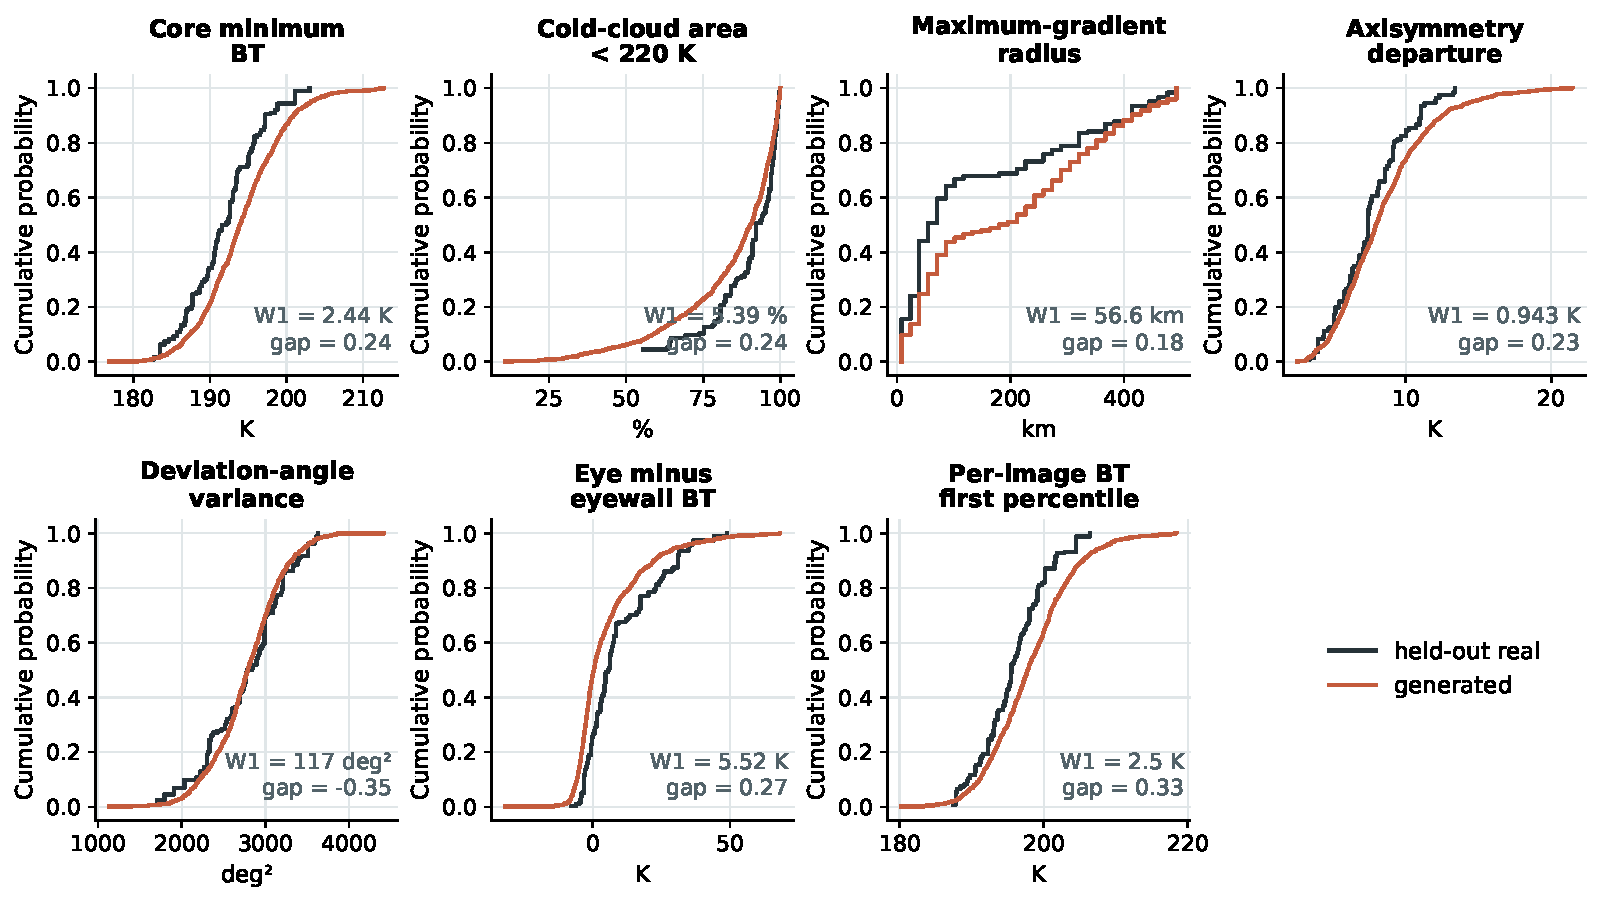
\includegraphics[width=17cm]{fig06.pdf}
\caption{Category 5 distributions for the seven physical quantities. Lines show the
event-balanced empirical cumulative distributions of held-out real storms and the
generated fields; the panel annotations give the native-unit Wasserstein distance and
reference gap. Category 5 contains only \CfiveFrames{} held-out images from
\CfiveStorms{} storms, so visual overlap and a within-reference-range label must be
read together with the thin-event behaviour in Figure~\ref{fig:validation}.}
\label{fig:c5dist}
\end{figure}

The same caution applies to spatial structure (Figure~\ref{fig:c5structure}). The
Category 5 radial profile and log-power discrepancy are within range, unlike the
log-power result for TS through Category 4. That contrast must not be interpreted as
evidence that the most intense storms are simulated more accurately. In the synthetic
experiment, the same 0.55-standard-deviation perturbation crossed in
\BalancedShiftCrossingRate{} of the 80-block trials but only
\CfiveLikeShiftCrossingRate{} in the 22-block design. Increasing the generated bank
to \GeneratedPerClass{} images does not create additional independent real storms.
The Category 5 range label is therefore supported by a less resolving reference, not
stronger evidence of fidelity. Its above-range feature-diversity result remains
visible rather than being averaged with Category 4.

\begin{figure}[t]
\centering
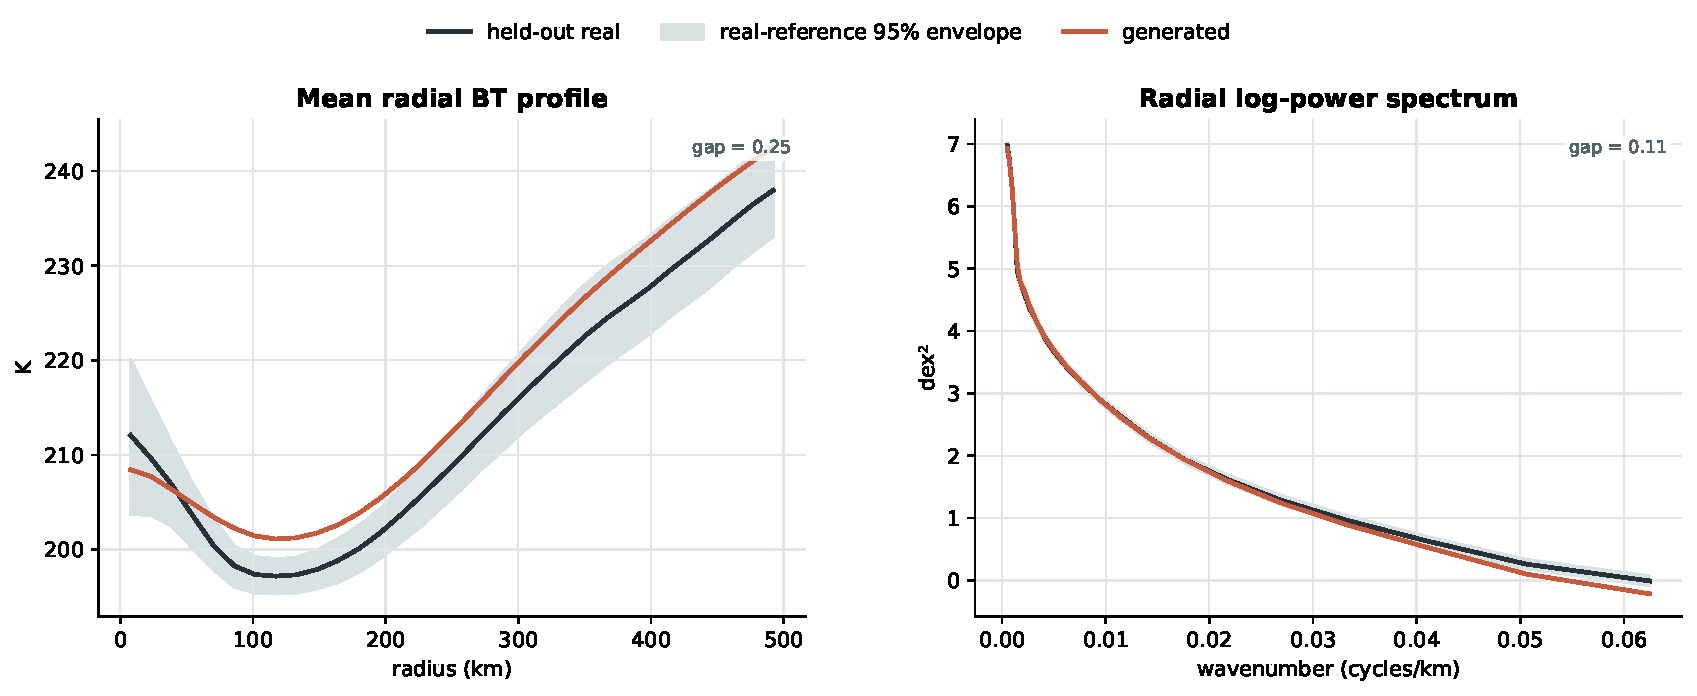
\includegraphics[width=17cm]{fig07.pdf}
\caption{Category 5 spatial-structure performance. The left panel compares radial
brightness-temperature profiles; the right compares Hann-windowed radial power
spectra. Neutral shading is the real-reference curve envelope; the generated curve
uses a distinct colour. The scalar discrepancies compare the complete curves rather
than counting visual excursions at individual radii or wavenumbers. The log-power
discrepancy is reported in dex\({}^2\).}
\label{fig:c5structure}
\end{figure}

\subsection{Metric controls, copying, and preprocessing}

The profile is interpretable only to the extent that its diagnostics respond to
relevant failures. The training-only controls therefore remain part of the result,
not a hidden implementation check. Temperature shifts move the core-minimum and
lower-tail distances monotonically; targeted warming and cooling around 220\,K move
the cold-cloud fraction; and the eye/eyewall perturbation moves eye contrast. Blur,
centre displacement, and radial deformation provide distinct responses for spatial
power, maximum-gradient radius, and radial profiles. The first reference crossing is
reported separately for every severity curve, so a monotone response that remains
inside the range is not mislabelled as a fully resolved control.

The structural and feature controls answer different questions. Phase randomisation
disrupts axisymmetry, deviation-angle variance, and the radial profile while
preserving each field's unwindowed Fourier magnitude to the registered numerical
precision. A 90-degree rotation remains inside the radial Hann-PSD reference range,
whereas blur and checkerboard artifacts move log-power as expected. In the exact
training-fitted feature representation, an EOF excursion controls MMD\({}^2\) and
density, mode removal controls coverage, and contraction and expansion control the
two directions of diversity. The full \ControlLaneCount-lane curves, invariance
checks, and metric-specific statuses appear in the Supplement.

Exact replay is recognized by the localized nearest-neighbour audit, and the
copied-fraction sweep establishes the smallest mixture resolved by this archive and
representation as \MinimumResolvedCopyFraction{}. The model-bank result must be read
with the sweep's design made explicit: the curve uses a
\ControlReferenceFields-field, event-disjoint
reserved-training comparison, whereas the model-bank audit searches the complete
\MemorizationTrainingFields-field diffusion-training archive. The
\MinimumResolvedCopyFraction{} point is therefore a response
demonstration, not a calibrated lower limit on copying in the model bank. The
model-bank result can describe supported feature neighbourhoods but cannot rule out
copying outside the registered representation. The separate preprocessing audit reports contact with the
generator's 170 and 325\,K clipping bounds; it is not presented as a test of physical
admissibility.

\subsection{Continuous-wind response and feature-space robustness}

The six native classes are the primary conditions, but a class label can still hide
whether the generator uses its continuous wind input. The post-hoc wind audit
therefore compares the within-class slope of every physical quantity for held-out
real and generated fields (Supplement). Real intervals resample storms and generated
intervals resample the fixed bank. We report these slopes as a response diagnostic,
without converting interval overlap into an equivalence verdict. Across the
\WindSlopeComparisons{} class--quantity combinations, the central interval excludes
zero for \WindRealResolved{} real slopes and \WindGeneratedResolved{} generated
slopes. Both archives resolve a non-zero response in \WindBothResolved{} cases, and
the estimated directions agree in all \WindBothSameSign{}. Category 5 illustrates
the role of observational support: \WindCfiveRealResolved{} of its real-data slopes
is resolved, whereas
\WindCfiveGeneratedResolved{} generated slopes are. Those generated responses show
that the conditioning input affects the bank, but the \CfiveStorms-storm real archive cannot
establish whether their magnitudes are representative.

The feature-space robustness audit similarly leaves the primary result unchanged. It
repeats MMD\({}^2\), density, coverage, and diversity across training-fit sizes, EOF
ranks, and low-pass spatial scales. The registered full-SVD representation remains
visually distinguished from the post-hoc alternatives. Across all
\FeatureRepresentationVariants{} representations, the
\FeatureRobustnessComparisons{} representation--class
comparisons per metric, MMD\({}^2\) and coverage remain within the empirical range in
\FeatureMmdWithinCount{} and \FeatureCoverageWithinCount{}, respectively. The
above-range diversity pattern persists in \FeatureDiversityAboveCount{}, but density
is above range in only \FeatureDensityAboveCount{}. Thus the MMD\({}^2\), coverage,
and elevated-diversity conclusions are comparatively robust, although the size of
the diversity gap changes; the density pattern should be described as
representation-dependent rather than as an intrinsic property of the generator.

\section{Discussion}
\label{sec:discussion}

The structured review shows that climate-generation studies use many scientifically
relevant diagnostics, but rarely connect them through a shared interpretation. In the
curated corpus analysed here, held-out test sets and conditional evaluation are common, yet
only about one fifth of papers quantify metric uncertainty, establish a real-vs-real
reference, or quantify diversity. Positive controls, physical-admissibility checks,
and memorization analyses are rarer still. Consequently, a paper can contain several
technically valid figures while leaving the reader unable to tell whether an apparent
model deficiency is larger than ordinary real-data variability or whether a reassuring
metric could have detected the relevant failure.

GAUGE does not propose a climate-specific replacement for FID or any other universal
image score. The physical quantities remain application-specific and retain their
native units. The contribution is the common comparison around them: the same sample
size, condition, event weighting, real-vs-real reference, uncertainty calculation, and
plain-language range description are applied to each metric. Diversity, preprocessing,
structural, and copying checks then prevent a small set of favourable
marginal distributions from standing in for the full generated distribution.

The framework extends the idea that model performance becomes meaningful only in
relation to appropriate benchmarks \citep{Seibert2018}. In hydrological modelling, a
calibrated and an uncalibrated version of the same bucket model can provide useful
upper and lower expectations. Generative climate applications lack an equivalent
common model, so GAUGE replaces literal bounds with two kinds of reference. Repeated
real-vs-real comparisons characterize the disagreement produced by this finite
archive and evaluation design, while deliberately degraded real data show how named
failure mechanisms appear under the selected metrics. The first is not an upper
performance bound, and the second is not a universal lower bound.

This distinction is why the reference-gap profile is deliberately not restricted to
zero and one. Gap zero means that the model discrepancy equals the median
real-vs-real discrepancy; gap one means that it reaches the 95th-percentile marker for this
evaluation. Neither value is a statement about scientific acceptability. Likewise, a
4\,K shift or two-pixel blur is a concrete diagnostic anchor, not the worst possible
generator. A zero-to-one normalisation based on those controls would change when the
chosen severity changed and would imply a false equivalence among different physical
failures. The unbounded gap instead provides a compact visual coordinate while leaving
scientific severity to the native-unit values.

The TC case illustrates the difference between plausible appearance and broader
distributional evidence. A conventional evaluation could present the generated
examples, overlapping physical cumulative distributions, and similar mean radial
profiles and conclude that the model is broadly realistic. GAUGE retains this
favourable evidence: each selected physical marginal and mean radial profile remains
within its class-specific reference range. At the same time, the log-power,
feature-density, and diversity patterns reveal discrepancies that the marginals do
not. These findings are not contradictory; they show that the generator reproduces
the selected physical distributions more successfully than it reproduces spatial
texture and feature-space dispersion.

The framework also prevents two misleading comparisons. First, the pooled experiment
reported in Section~\ref{sec:results} and the Supplement makes the model
appear poor because the generated bank is class balanced and the real test set is not.
The separate class results show that this discrepancy is primarily a composition
question. Second, the Category 5 results appear favourable but are based
on only \CfiveStorms{} independent real storms. The real-reference distribution and
Monte Carlo validation make that limitation visible: a within-range label in Category
5 comes from a less resolving archive than the same label in a class supported by
many more storms.

GAUGE is complementary to, rather than competitive with, established forecast
verification. CRPS, reliability diagrams, rank histograms, FSS, and SAL exploit
pairing, ensemble membership, location, scale, or object correspondence. Version 0.2
addresses a different question: whether an unpaired bank of independent generated
fields reproduces selected properties of a real field population. When both
questions arise, both forms of evidence are needed. Similarly, common benchmark
suites provide external comparability accumulated across models, whereas GAUGE
constructs study-specific context when no shared analysis-ready benchmark exists.

The protocol is also modular in computational cost. Scalar functionals and their
event-aware real references are inexpensive and form the interpretable core.
Quadratic feature metrics, large control suites, and representation-robustness audits
are more demanding and should be selected because they address a plausible failure,
not because the framework requires every available diagnostic. What is mandatory is
that each reported result states its data support, weighting, reference construction,
uncertainty meaning, and control status.

\subsection{Limitations}

The statistical conclusions are deliberately bounded. The selected 95th percentile
is an empirical marker, not an analytical error-rate guarantee. The simulation study
characterizes same-population crossings and response to known changes only for the
examined distributions and event structures. A different dependence process,
archive, metric, or block definition can produce different behaviour. In particular,
GAUGE can validate identifiers syntactically but cannot determine whether a storm,
year, member, or other label is the scientifically correct independent unit.

The central comparison range holds the generated bank fixed while changing the
admissible held-out-real subset. Its paired-bootstrap interval describes numerical
Monte Carlo precision, and the grouped deletion experiment probes sensitivity to the
available real events. Neither includes generator retraining, a new sample bank, or a
new observational archive. Algorithm-level repeatability claims therefore require
additional model fits or banks outside the v0.2 report.

The scientific scope is similarly explicit. Feature diagnostics can miss failures
outside their training-derived representation, and the copying test is limited to its
supported feature neighbourhoods and demonstrated copy fractions. GAUGE records
physical definitions and controls but cannot determine which field properties matter
for every application.
The present implementation evaluates independent generated fields; temporal
coherence, coupled-variable constraints, and forecast calibration require registered
metrics and sampling designs for those settings. The TC study demonstrates one
generator and field type, and its limited Category 5 observations do not establish
Category 5 fidelity. The wind-response and feature-space robustness analyses are
post-hoc diagnostics, not alternative endpoints. Moreover, GAUGE and the TC analysis
were refined after the held-out archive had informed earlier development; the
versioned amendment log makes that history explicit, but the demonstration is not a
pristine confirmatory experiment. Finally, the review counts describe the curated
69-paper corpus, not field-wide prevalence.

\conclusions

Our review of 69 climate-generation studies shows that evaluation practice has
expanded rapidly but remains fragmented: held-out and conditional comparisons are
common, while uncertainty, real-vs-real references, diversity, metric validation,
physical checks, and memorization are documented much less often. GAUGE turns
these separate concerns into a coherent and interpretable protocol. It combines
application-defined physical quantities with structural, feature-space,
admissibility, and copying diagnostics; keeps correlated events separate across the
two real samples; and evaluates every model discrepancy against the disagreement
observed between those matched samples.

The TC demonstration avoids both an undifferentiated success claim and an
undifferentiated failure claim. Its selected physical distributions and mean radial
profiles lie within their class-specific real-reference ranges, while spatial
log-power and feature-space diagnostics expose a different pattern of structural and
dispersion discrepancies. The same analysis shows that Category 5 evidence is limited
by only \CfiveStorms{} independent storms and that a pooled result is confounded by
the different intensity mixtures.
GAUGE's principal contribution is therefore not a score for this diffusion model. It
is a practical way to state which properties were measured, how each observed
discrepancy compares with finite real-data variation, whether the metrics respond to
known failures, how sensitive a pattern is to representation choices, and where the
available archive leaves the comparison weakly resolved. The
complete class-by-metric results, control-severity curves, robustness analyses, and
provenance audits are provided in the separately compiled Supplement.

\codedataavailability{The GAUGE source code, statistical-validation harness,
literature-review coding pipeline, TC configurations, checksummed manifests,
machine-readable evaluation report, and scripts that regenerate every manuscript
figure and table are available at
\url{https://github.com/gascenso/climategen-eval} as version 0.2.0. Persistent
identifiers for the immutable software release and the permission-cleared archive of
derived TC fields and the generated bank will be inserted after the deposition
workflow is complete. GridSat-B1 and IBTrACS are available from their NOAA source
services and are described by \citet{Knapp2011} and \citet{Knapp2010},
respectively.}

\authorcontribution{GA conceived the study, designed the protocol, implemented and
validated the software, curated and analysed the case-study and literature-review
data, produced the figures, and drafted the manuscript. AC supervised the work and reviewed and edited the manuscript.}

\competinginterests{The authors declare that there is no conflict of interest.}

\begin{acknowledgements}
OpenAI Codex was used to assist with figure and table assembly and language drafting. The authors reviewed the source material and take responsibility for the manuscript and all scientific claims.
\end{acknowledgements}

\begingroup
\hbadness=10000
\bibliographystyle{copernicus}
\bibliography{references}
\endgroup

\end{document}
